\chapter{Methode}
\label{chapt:Methode}
\section{Fragestellung}
Aus diesem Grund stellt sich die Frage, ob sich genetische Algorithmen zur Optimierung von Obfuskatorkaskaden unter den Kriterien die für praktische Red Team Assignments relevant sind, als Werkzeug nutzen lassen. Diese Frage speist sich zum einen aus der ungeheuren Prävalenz von Obfuskatoren und Packern in der Bedrohungslage (QUelle: ?) und auf der anderen Seite den zeitlichen und zum Teil auch ressourcenbedingten Begrenzungen, die ein Red Team einhalten muss. 

-----------------------

----------------------------------

Durch Obfuskation steigt zum einen die Größe der Datei und die Entropie innerhalb der Datei, was beides Faktoren sein können, die von AV-Software erkannt und betrachtet werden können.



\section{Kriterien}
Für die praktische Verwendung muss ein solches Tool möglichst autonom und erweiterbar sein. Des weiteren ist es wichtig, dass es innerhalb der 


\section{Verwendete Technologie}
\subsection{Architektur}
Für die Entwicklung der zwei Modi (Dropper und PE File) wurde die Architektur für den genetischen Algorithmus entsprechend angepasst. In \ref{fig:architecture} sieht man die vollständige Architektur, die mittels AWS Services aufgebaut wurde. Sie beinhaltet die AV Scanner und Obfuscator in ihren eigenen Instanzen und den Genetischen Algorithmus in seiner eigenen Instanz. Für die Obfuskation von PE Files werden diese erst an die Obfuskator gesendet, zwischengespeichert und anschließend an die AV Scanner gesendet. Bei dem Shellcode Dropper wird die gleiche Dropper Executable an den AV Scanner gesendet, welcher dann den obfuskierten Shellcode von einem Webserver der GA Instanz herunterlädt und ausführt, während er gescannt wird.
\begin{figure}[h]
    \centering
    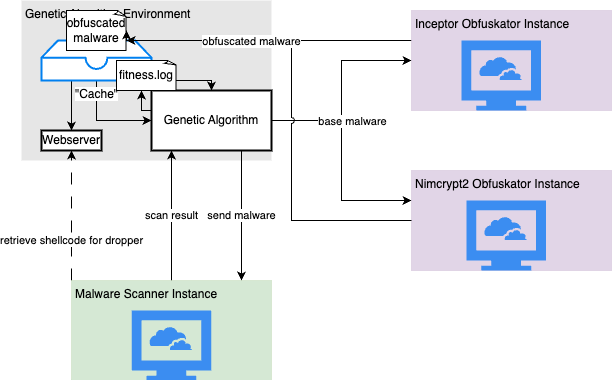
\includegraphics[width=0.85\textwidth]{gfx/Abbildungen/Architektur.drawio.png}
    \caption{Architektur von Obscurus Evolved}
    \label{fig:architecture}
\end{figure}\section{Genetischer Algorithmus im Detail}
    \subsection{Suchproblem Formalisierung}
    Um einen genetischen Algorithmus für ein Problem sinnvoll zu verwenden, muss zuerst einmal ein zugrunde liegendes Problem als Suchproblem formuliert werden. Im vorliegenden Anwendungsfall würde eine solche Formalisierung daraus bestehen.


Sei $K = \{e_1, e_2, \ldots, e_n\}$ eine Menge von Elementen, wobei jedes Element $e_i$ entweder vom Typ $O$ oder $E$ ist. Gesucht ist eine Konfiguration $K$, sodass die Funktion $f(K)$ maximiert wird.

\begin{comment}

\end{comment}
\section{Gütekriterien und Definition}
Eine Obfuscation ist dann gut, wenn sie von AV nicht erkannt wird, ausführbar ist und noch ihren Zweck erfüllt. Eine langsame Erkennung durch AV wird ihr positiv angerechnet. Ein Durchlauf eines Genetischen Algorithmus ist gut, wenn er eine Anzahl von guten Obfuskationen > 0 erzeugt und eine geringe Gesamtlaufzeit hat.
\section{Red-Teaming Kriterien}
Aufgrund der Anforderungen, die im Red Teaming relevant sind, dürfen Sachen nicht ewig lange dauern und dürfen nicht spezifisch auf gegebene Betriebssysteme, Techniken, AV Software zugeschnitten sein.

\section{Verwendete Technologien}
    \subsection{Pipeline}
    Obscurus = Internes SAP Tool/Framework zum API Basierten Obfuskieren von Exe und RAW Payloads mittels Obfuskator und Konfiguraionen, sowie einem 
    \subsection{Obfuskatoren}
    Nymcrypt2 und Inceptor
    \subsection{Antivirenscanner}
    Microsoft Defender stuff

\section{Genetischer Algorithmus}
Der vorhandene genetische Algorithmus wurde auf Basis des vorliegenden Problems mit 2 Obfuskatoren entwickelt und dafür optimiert. Einige Entscheidungen für spezifische genetische Operatoren wurden mittels eines Pretests getroffen.

\subsection{Encoding}
Die Lösungskandidaten bestehen aus einer Liste von Obfuskator Konfigurationen. Diese Obfuskatorkonfigurationen beinhalten jeweils alle Eigenschaften, die für jeden der Obfuskatoren als Optionen nötig sind, und benutzen die Eigenschaften, die für den ausgewählten Obfuskator nötig sind. Dies hat zwar zur Folge, dass es starke epigenetische Effekte\footnote{Veränderung eines Genes, die kaskadierende Auswirkungen auf die restlichen Gene im Kandidaten hat} geben und Mutationen völlig ergebnislos bleiben, ermöglicht dafür aber die sinnvolle Verwendung von diversen Rekombinationsarten. Konzeptionell besteht das Encoding damit also aus einem String von gequantelter Größe, die allerdings nicht konstant ist. 
In genetischen Algorithmen ist es eher ungewöhnlich, dass die Länge eines Lösungskandidaten ungleich der von anderen ist, was bei der Rekombination zu Problemen geführt hat. Die Entscheidung für dieses Design liegt darin, dass der Algorithmus von selbst die optimale Obfuskationslänge entscheiden soll und zeitgleich möglichst laufzeiteffizient werden soll.
\begin{figure}[h]
    \centering
    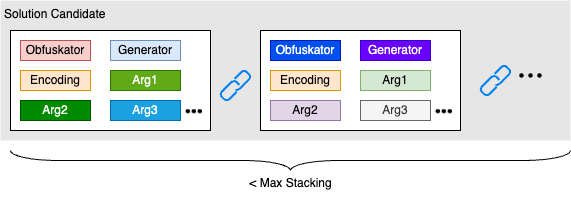
\includegraphics[width=0.85\textwidth]{gfx/Abbildungen/Encoding Diagram.png}
    \caption{Encoding Darstellung}
    \label{fig:encoding}
\end{figure}
\subsection{Selektion}
Für die Selektion wurde im Algorithmus auf die sogenannte Turnierselektion zurückgegriffen, die neben der einfachen Programmierbarkeit es auch leicht macht, den Selektionsdruck anzupassen. \cite{blickle_1996_a} (1995 Tournament Selection and Noise). Ein weiterer Vorteil dieses Verfahrens ist es, dass man nicht die Fitness aller mutierten und rekombinierten Kandidaten einer Population berechnen muss, sondern nur derjenigen, die in einem Turnier teilnehmen. Als weitere Ergänzung und Laufzeitoptimierung kommt der sogenannte "David"-Parameter zum Tragen, welcher dem unterlegenen Kandidaten in einem Turnier als Sieger hervorgehen lässt und so die Diversität der kommenden Generation erhöhen kann.

\subsection{Mutation}
\begin{figure}[h]
    \centering
    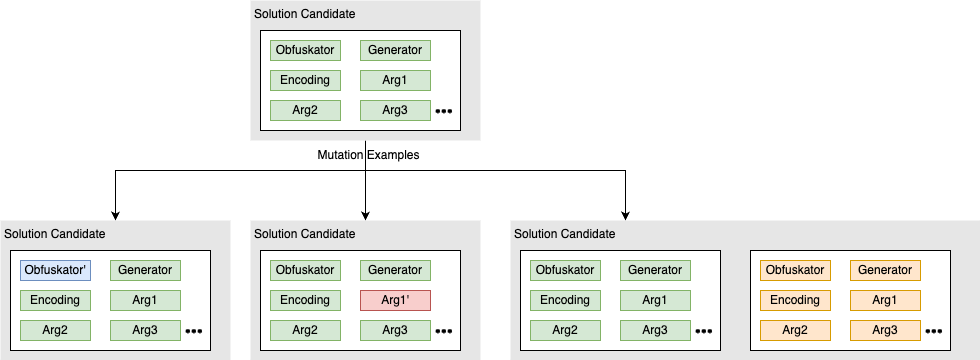
\includegraphics[width=0.85\textwidth]{gfx/Abbildungen/Mutations.png}
    \caption{Mutationsmöglichkeiten}
    \label{fig:mutations}
\end{figure}
Die Mutation ist in zwei Bestandteile aufgeteilt. Einerseits eine simple Veränderung einer Obfuskatorkonfiguration innerhalb des Lösungskandidaten und damit innerhalb der Liste. Andererseits das Hinzufügen von einer zufälligen neuen Obfuskatorkonfiguration in den Lösungskandidaten, um so eine längere Lösung zugänglich zu machen.


\subsection{Rekombination}
Für die Rekombination sind viele verschiedene Implementierungen möglich gewesen. Nach einigen Überlegungen wurden dann zwei verschiedene Rekombinationsarten implementiert und ausprobiert.
\subsubsection{String-based-Recombination}
Ähnlich dem klassischen Binary-String Encoding werden hier die Lösungskandidaten an einer beliebigen Stelle durchgeschnitten und die zweite Hälfte zwischen diesen ausgetasucht. Dieser Schnitt kann selbstverständlich an einer Obfuskationskonfigurationsgrenze auftreten und so nur das Stapeln verändert, aber auch innerhalb der Konfiguration.
\subsection{Sacrifice Based Shema}
In diesem Beispiel wird von einem Kandidaten eine Konfiguration entfernt und dem anderen Kandidaten hinzugefügt. Dies kann dazu führen, dass eine Lösung keine Obfuskationsschritte beinhaltet und dabei dann als nicht obfuskiertes File behandelt und gescanned wird.

\subsection{Fitness Funktion}
Die Fitness Funktion setzt sich aus mehreren Faktoren zusammen und lässt sich nicht einfach als richtig oder falsch definieren sondern basiert stark auf dem zugrundeliegenden Optimierungsproblem. Das vorliegende Beispiel geht etwas über das Problem von klassischen genetischen Algorithmen hinaus, indem es nicht nur die Kandidaten optimieren soll, sondern zeitgleich auch noch die Laufzeit des gesamten Algorithmus möglichst kurz halten (Hyperparameter).
In diesem Fall gibt es die folgenden Faktoren:

\subsubsection{Obfuskations und Detektions-Dauer}
Wie lange braucht es die die obfuskierte Malware in all ihren Schritten zu erzeugen unter Verwendung von Cashing. Dies ist einer der genannten Hyperparameter, da die gesamte Laufzeit des Algorithmus sich aus der Summe von durchgeführten Obfuskations und Detektionszeiten zusammensetzt und eine Population, die aus Kandidaten besteht, die nur kurze Obfuskations und Detektionsdauern hat, zu einer kürzeren Laufzeit beiträgt. $t_O,  t_D$
\subsubsection{Obfuskationsschritte}
Die Anzahl an Obfuskationsschritten, die der Kandidat behinhaltet. Dies hängt auch stark mit ((!TODO!)) der initalen Population von Kandidaten zusammen und wie diese gestapelt ist. $N_O$
\subsubsection{Detektionsergebnis}
Die Ergebnisse des Scanners, ob die Datei als Malware erkannt wurde und ob der Scanner sie überhaupt durchführen konnte und damit lauffähig ist. $D_{Malicious}=1, D_{Benign}=10^5$

\subsubsection{Funktion}
Die Funktion zeichnet sich durch die oben genannten Hyperparameter aus. Diese sollen zwar nicht für die einzelnen Kandidaten entscheidend sein, dennoch einen Einfluss auf die Gesamtheit der Population haben.

Der Primäre Zweck der Funktion ist es, Malware so zu obfuskieren, dass sie nicht erkannt wird. Sekundär soll dabei die Laufzeit des gesamten Algorithmus klein gehalten werden. Dies kann zu einem Teil durch die Fitnessfunktion bewerkstelligt werden, zum anderen über Caching, welches durch die Fitnessfunktion belohnt werden soll. Andererseits soll für die Analyse der wissenschaftlichen Fragestellung die Verwendung von mehrstufigen Obfuskationen befürwortet werden. Eine Möglichkeit dies zu gewährleisten ist es, dass man die Obfuskationszeit von gecachten nicht künstlich erhöht und nachhält, sondern nur die tatsächlich verbrauchte Zeit bis zum fertig obfuskierten Payload gemessen wird und als $t_O$ interpretiert wird.
Ein weiterer Ansatz, um das Gleichgewicht zwischen Minimierung von Laufzeit und Diversität der Lösungslängen zu wahren, wäre eine T/Z-Transformation der Obfuskationszeiten mit einer angenommenen $\sigma _{t_D}=5s$ und $\overline{M_{t_D}}$

$\frac{D_{Benign, Malicious}}{t_D}+t_O$


\subsection{Experiment}
\section{Hypothesen}
Im Anbetracht der Fragestellung lassen sich schon im Vorfeld einige Vermutungen anstellen, die im Folgenden dargelegt werden sollen.
\subsection{PE-Files}
\textit{Mindestens 5\% der mehrfach obfuskierten PE Files sind korrumpiert und nicht ausführbar.}
Mehrfach obfuskierte PE Files werden wahrscheinlicher von AV-Software entdeckt und/oder anfälliger für Dateikorrumpierung.
PE Files sind lore Ipsum dolor sit. ihre Struktur bla blablabal
\subsection{Shellcode}
\textit{Mehrfach obfuskierter Shellcode ist in weniger fällen als die PE Files korrumpiert und nicht ausführbar.}
Hier wird davon ausgegangen, dass der Shellcode an sich schon signifikant kleiner ist als ein PE File und eine kleine Veränderung in einer Operation nicht zwangsläufig die Veränderung des gesamten Files korrumpiert.
\subsection{Kriterien}
\textit{Der vorgeschlagene Genetische Algorithmus ist in der Lage die Anforderungen an Laufzeit und Ergebnisse des Red-Teamings zu erfüllen.}
\subsection{Multi Obfuscated}
\textit{Die Anzahl der Obfuskationsschritte hat einen Einfluss auf die Erkennungswahrscheinlichkeit der Payload.} (Positiv, negativ o.ä. Als einzelne Gruppen interpretieren je nach Länge)
\subsection{Shell Access}
\textit{Evaded Shellcode Zeug führt in weniger als 50\% der Fälle zu tatsächlichem Shell Access}